% !TeX program = lualatex
% !BIB program = biber
% Andamiaje. No es la prosa final. Compiler: LuaLaTeX. Bibliografía: Biber.
\documentclass{ucaldas-tesis}
\addbibresource{references.bib}

% Generado por scripts/v3/exportar_cifras_tesis.py. No editar a mano.
\newcommand{\FraseSuero}{No se detecta diferencia; 166 proteínas son equivalentes}
\newcommand{\TitularMl}{La separación del suero entre cáncer y colonoscopia negativa se explica por la calidad de muestra.}
\newcommand{\ClaveTitular}{separacion\_explicada\_por\_calidad}
\newcommand{\SueroN}{284}
\newcommand{\SueroDiferente}{0}
\newcommand{\SueroEquivalente}{166}
\newcommand{\SueroIndeterminada}{118}
\newcommand{\Huno}{rechaza\_h1}
\newcommand{\Runo}{147/147}
\newcommand{\HunoFragil}{False}
\newcommand{\Hcinco}{refuta}
\newcommand{\Hsiete}{refuta}
\newcommand{\Hdiez}{descriptiva}
\newcommand{\HdiezN}{5}
\newcommand{\Advertencia}{Ningún resultado de esta tesis sirve para decidir sobre un paciente.}

\begin{document}

\thispagestyle{empty}
\begin{center}
\vspace*{2.2cm}
{\fontsize{16}{20}\selectfont\bfseries Qué parte del tumor colorrectal se deja ver en la sangre\par}
\vspace{1.8cm}
{\fontsize{14}{18}\selectfont Juan Diego Polanco Franco\par}
\vspace{1.8cm}
{\fontsize{14}{18}\selectfont Universidad de Caldas\par}
\vspace{0.8cm}
{\fontsize{12}{16}\selectfont Facultad de Inteligencia Artificial e Ingenierías\par}
\vspace{1.6cm}
{\fontsize{12}{16}\selectfont Manizales, Colombia\par}
\vspace{0.4cm}
{\fontsize{12}{16}\selectfont 2026\par}
\end{center}
\clearpage

\thispagestyle{empty}
\begin{center}
\vspace*{1.2cm}
{\fontsize{16}{20}\selectfont\bfseries Qué parte del tumor colorrectal se deja ver en la sangre\par}
\vspace{1.2cm}
{\fontsize{14}{18}\selectfont Juan Diego Polanco Franco\par}
\vspace{1cm}
\begin{minipage}{0.92\textwidth}
\centering
Tesis o trabajo de investigación presentada(o) como requisito parcial para optar al título de:\par
\vspace{0.4cm}
Magíster en Bioinformática y Biología Computacional\par
\vspace{0.3cm}
\fontsize{10}{13}\selectfont
Programa de investigación, 60 créditos, SNIES 103917.\par
Convenio SUMA con la Universidad de Manizales, la Universidad Autónoma de Manizales y la Universidad Católica de Manizales.\par
\normalsize
\end{minipage}
\vspace{0.9cm}
\end{center}
\noindent Director:\par
Doctor en Ingeniería, Jorge Alberto Jaramillo Garzón\par
\vspace{0.4cm}
\noindent Grupo de investigación:\par
Grupo de Investigación en Tecnologías de la Información y Redes (GITIR)\par
\vspace{0.4cm}
\noindent Línea de investigación:\par
Modelos Computacionales y Bioinformática\par
\vspace{1.2cm}
\begin{center}
Universidad de Caldas\par
Facultad de Inteligencia Artificial e Ingenierías\par
Manizales, Colombia\par
2026\par
\vspace{0.6cm}
{\fontsize{10}{12}\selectfont\textit{Andamiaje, 11 de noviembre de 2026. No es la prosa final.}\par}
\end{center}
\clearpage

\chapter*{Declaración de uso de herramientas de inteligencia artificial}
\addcontentsline{toc}{chapter}{Declaración de uso de herramientas de inteligencia artificial}
\objetivo{Declarar qué herramienta se usó, con qué versión o fecha, para qué y hasta dónde. Ninguna de estas herramientas es fuente de un hecho científico.}
\todojd{Reescribe la tabla con tus palabras si quieres cambiar el propósito o el alcance. La versión y la fecha ya están.}

\begin{table}[ht]
\caption{Herramientas de inteligencia artificial usadas en el trabajo}
\label{tab:ia}
\begin{tabular}{p{3.2cm}p{3.4cm}p{3.6cm}p{3.4cm}}
\toprule
Herramienta & Versión o fecha & Propósito & Alcance \\
\midrule
Cursor (Anysphere) & 3.28.7 & Escribir y depurar código & El autor revisó, ejecutó y validó el código \\
SciSpace & Consultado entre 2026-03 y 2026-11 & Buscar y hacer un primer filtro de literatura & No sustituye la lectura del artículo \\
\bottomrule
\end{tabular}
\end{table}
\fuente{Declaración del autor. No es un resultado de \texttt{results/v3\_7/}.}

\todojd{Ajusta este párrafo.}
Se utilizó Cursor (Anysphere) como asistente de programación para escribir y depurar código, y SciSpace como apoyo para buscar y hacer un primer filtro de literatura científica. El código, los resultados y las fuentes fueron revisados, ejecutados y validados por el autor, quien asume la responsabilidad total del contenido. \cite{cursor2026,scispace2026}
\clearpage

\chapter*{Resumen}
\addcontentsline{toc}{chapter}{Resumen}
% fuente: results/v3_2/k1_etiquetas.json
% fuente: results/v3_2/suero_resumen.json
% fuente: results/v3_2/k5_auc.json
% fuente: results/v3_2/k7_control_tecnico.json
% fuente: results/v3_2/hipotesis_v3_2.tsv
El cambio proteico del tumor colorrectal ya está descrito en el tejido. Esta versión pregunta qué parte de ese cambio es propia del colon y cuál llega a la sangre. No se fusionaron cohortes. En el contraste no se imputaron ausencias. El ancla fue el proteoma TMT de CPTAC, PDC000116: 688 proteínas de 7\,394 cambian al menos 1,5 veces, con tasa de descubrimientos falsos de 0,05. La réplica fue PXD034575, 16 pacientes. P es el tumor primario, M la metástasis hepática y N la mucosa. Una lectura anterior tomó M como tumor y obtuvo 104 de 119 signos iguales. La corrida vigente excluye 237 filas de contaminante o señuelo y pide al menos ocho pares. El primario frente a la mucosa coincide en 89 de 90, con intervalo de 0,940 a 0,9997 y concordancia de Lin 0,704. La metástasis frente a la mucosa coincide en 69 de 82, con Lin 0,390. La detectabilidad por péptido único, 226 de 688, no cambia con la etiqueta.

El suero fue PXD055218, 20 personas por grupo. El informe trae 897 grupos. Con FDR de proteína del 1\,\% y especie humana quedan 312. El contraste oficial, sin contaminantes ni paneles de calidad, tiene 205 proteínas. Frente a la colonoscopia negativa, ninguna es diferente, 105 son equivalentes y 100 quedan indeterminadas. La ausencia solo se afirma en las 105. Frente a personas sanas se separan SAA1 y LBP. CHMP4A no entra: su q global de grupo es 0,037. El máximo del área bajo la curva, ya sin contaminantes ni paneles, es 0,865 en SERPINA3; con 10\,000 permutaciones, p = 0,0464. En la matriz humana sin esa limpieza el máximo es 0,939, en FGB. La piel y la coagulación difieren entre grupos. H5 no se pudo calcular y H10 cuenta cero proteínas específicas de 1\,165, sin un veredicto fijado de antemano. El trabajo no propone un examen de sangre.

\noindent\textbf{Palabras clave:} cáncer colorrectal; proteómica; suero; especificidad; Gene Ontology; neoantígeno.
\clearpage

\begin{otherlanguage}{english}
\chapter*{Abstract}
\addcontentsline{toc}{chapter}{Abstract}
% fuente: results/v3_3/certificado_v3_3.json
% fuente: results/v3_3/suero_resumen.json
% fuente: results/v3_3/k1_etiquetas.json
The protein change of the colorectal tumor is already described in tissue. Run v3.3 asks whether that change reaches the blood and whether serum separates cancer from a negative colonoscopy. Cohorts were not merged. Missing values were not imputed in the contrast. The anchor is the 688 certified CPTAC proteins. The replicate is PXD034575, 16 patients. P is the primary tumor, M the liver metastasis and N the mucosa.

The run drops 237 contaminant or decoy rows and requires at least eight pairs. Primary versus mucosa agrees in sign for 147/147, with an interval from 0,975 a 1 and Lin concordance 0,770. Metastasis versus mucosa agrees for 116/143, with Lin concordance 0,434. CA1 falls in the tumor. AQP8, SLC26A3 and GUCA2A have no log2 fold change, so the tissue labels are not confirmed.

Serum is PXD055218, 20 people per group. The report has 897 groups. A 1\% protein false-discovery rate and the human species filter leave 312. The principal contrast has 284 proteins: 0 different, 166 equivalent and 118 indeterminate against the negative colonoscopy. Against healthy people the separated proteins are LRG1 (P02750), SAA1 (P0DJI8), LBP (P18428). The separation seen by the model is explained by sample quality. H5 is refuta and H7 is refuta. H10 is descriptiva and counts 5 specific proteins. The work does not propose a blood test.

\noindent\textbf{Keywords:} colorectal cancer; proteomics; serum; specificity; sample quality.
\end{otherlanguage}
\clearpage

\tableofcontents
\cleardoublepage
\listoftables
\cleardoublepage
\listoffigures
\cleardoublepage

\chapter*{Lista de abreviaturas}
\addcontentsline{toc}{chapter}{Lista de abreviaturas}
\todojd{Revisa cada fila y borra la que no uses en la prosa.}
\begin{longtable}{@{}p{2.4cm}p{11.5cm}@{}}
\toprule
Sigla & Significado \\
\midrule
\endhead
AUC & área bajo la curva \\
BH & Benjamini-Hochberg \\
CN & colonoscopia negativa: pacientes sintomáticos con otra enfermedad intestinal \\
CP & colonoscopia positiva \\
CPTAC & Clinical Proteomic Tumor Analysis Consortium \\
DIA & adquisición independiente de datos \\
FDR & tasa de descubrimientos falsos \\
GO & Gene Ontology \\
HC & grupo medido aparte; no es el contraste que decide la pregunta \\
LFQ & cuantificación sin marcaje \\
NES & puntuación de enriquecimiento normalizada \\
PRM & monitoreo paralelo de reacciones \\
TMT & marcado isobárico en tándem \\
TOST & dos pruebas unilaterales \\
TREAT & prueba de equivalencia con un margen de cambio \\
\bottomrule
\end{longtable}
\clearpage

\mainmatter
\chapter{Introducción}
\objetivo{Plantear el problema, la justificación, la pregunta y los objetivos, sin prometer un examen de sangre.}
\todojd{Redacta de 2 a 4 páginas. La guía de 2022 deja el planteamiento, la justificación y los objetivos dentro de la introducción, no como capítulos propios. Por eso este andamiaje no abre un capítulo para cada uno.}

\section{Campo y problema}
\begin{itemize}
\item El tejido publicado ya describe el tumor y la mucosa. \cite{vasaikar2019,zhang2014,tanaka2024}
\item El suero es otra matriz y otras personas. El depósito que lee esta tesis es PXD055218. \cite{rai2025}
\item CN no son personas sanas. HC se midió aparte y no decide la pregunta.
\end{itemize}
\todojd{Responde: qué se conoce del cáncer colorrectal en tejido y qué parte de ese problema aborda esta tesis. No localices las muestras en un segmento del colon.}

\section{Justificación}
\begin{itemize}
\item La equivalencia estadística no es identidad biológica. El cero de la clase diferente no dice que el tumor no cambie en el tejido.
\item No hay una cohorte nueva medida. Las redes de coexpresión no se calcularon.
\end{itemize}
\todojd{Escribe por qué la pregunta merece el trabajo y qué hueco no reclamas como prioridad.}

\section{Pregunta}
Qué parte del cambio del tumor se deja ver en la sangre cuando el contraste es otra enfermedad intestinal.
\todojd{Deja la pregunta en una frase y, en otra, sus límites: matrices separadas, sin examen clínico.}

\section{Objetivos}
\todojd{Redacta un objetivo general y los específicos en infinitivo. Una conclusión del capítulo 6 debe poder responder a cada específico.}
\begin{itemize}
\item General, a partir de la pregunta de arriba. No lo dejes como una promesa diagnóstica.
\item Específicos que el repo sí puede sostener: concordancia de signo en tejido (\TejidoNum\ de \TejidoDen); celda del suero (\SueroDif, \SueroEq, \SueroInd, de \SueroN); calidad de muestra y orden de adquisición; estado de H5 a H10.
\end{itemize}

\section{Alcance}
\begin{itemize}
\item Trabajo \textit{in silico} sobre datos públicos. No propone un examen clínico. \cite{pepe2001}
\item Certificado: \CertificadoEstado. Sello \texttt{71b310a3fcaebe9267fac971156df3aab491e009}, 2026-11-11T00:48:45Z. Etiqueta \texttt{v3.7-final} en \texttt{595118ae09ea6006c744c86b28cb0a10d42e0442}.
\end{itemize}
Citas sugeridas: \cite{vasaikar2019,tanaka2024,rai2025,garciafoncillas2026,pepe2001}.
Extensión orientativa: 2 a 4 páginas para todo el capítulo.

\chapter{Marco teórico}

\section{Qué mide cada técnica}
El tejido de CPTAC llega marcado con TMT. Varias muestras se comparan dentro del mismo experimento y el archivo ya está en log2 \parencite{vasaikar2019}. El tejido de \textcite{tanaka2024} es LFQ: la intensidad de cada proteína se estima en cada muestra por separado, con MaxQuant. El suero de \textcite{rai2025} es DIA: se intentan ver muchas proteínas a la vez, sin elegirlas de antemano, y el informe las entrega en grupos. El PRM de ese mismo estudio, cuatro péptidos, es una medición dirigida que aquí no se reanaliza. \textcite{lesur2023} miden un panel dirigido de plasma. Esas columnas no entran en el contraste, porque un orden alfabético de los archivos no es un diagnóstico.

\section{Cómo se lee un cambio de abundancia}
En MaxQuant, el cero significa que la proteína no se identificó en esa muestra \parencite{cox2008}. Tratar el cero como cantidad cero hunde la mediana y hace creer que la matriz ya está en logaritmo. Por eso el cero se vuelve un hueco y solo la intensidad positiva pasa a log2. Un log2FC de 1 es el doble. Un log2FC de $-1$ es la mitad.

\textcite{smyth2004} modera la varianza entre proteínas para que una medición escasa no se declare distinta solo porque su desviación salió pequeña. \textcite{mccarthy2009} llaman treat a la prueba contra un cambio mínimo, no contra cero. \textcite{benjamini1995} controlan la fracción esperada de falsos entre las proteínas que se declaran distintas. El corte usado es 0,05. El área bajo la curva ordena personas: 0,50 es el azar. No dice si la proteína sube o baja y no sustituye a la tasa de descubrimientos falsos.

En el tejido de Tanaka, tumor y mucosa son de la misma persona: el contraste resta dentro de la persona. En el suero, los grupos son personas distintas: el contraste compara grupos. Pedir pareo donde no hay pares inventaría una relación.

\section{Gene Ontology y fichas}
\textcite{ashburner2000} proponen Gene Ontology como vocabulario de procesos, componentes y funciones. \textcite{subramanian2005} proponen mirar si los genes de un proceso se acumulan al principio de un ranking, no solo si un gen pasa un corte. Un suero que mide pocos genes de cada proceso no puede declarar que el proceso del tumor está en la sangre.

\textcite{uhlen2015} publican concentraciones de referencia en sangre. Esas concentraciones no son las de estos pacientes. \textcite{jumper2021} predicen un pliegue con AlphaFold. Un pliegue no demuestra que la cantidad haya cambiado. La ficha de cada proteína reúne el acceso de UniProt, los términos GO, la anotación de secreción y esos dos enlaces para que otra persona pueda verificar la fila.

\section{Neoantígenos}
Un neoantígeno es un péptido cuya secuencia cambió por una mutación y que el tumor puede presentar. \textcite{rai2025} describen 19 péptidos en suero y validan cuatro por PRM, uno de ellos neoantigénico. \textcite{xiang2026} identifican 96 neoepítopos mutados de MHC-I en tejido de diez pacientes; la mayoría proviene de regiones no codificantes. \textcite{hembrough2026}, en un resumen de congreso, recuperan cinco péptidos de una persona con cáncer colorrectal avanzado, desde vesículas de plasma. Ninguno de esos trabajos se convierte en una fila de abundancia de esta tesis. La matriz guarda grupos de proteínas, no la letra mutada.

\section{Estado del arte que cambia la lectura}
\textcite{tanaka2024} describen tripletes de tumor primario, metástasis hepática y mucosa. La columna P de esa matriz es el primario, no un pólipo. \textcite{ogren2026} publican un panel de plasma para cáncer colorrectal formado por CEACAM5, FLT1, IL19 y ferritina. \textcite{verathamjamras2023} encuentran la fibronectina más baja en plasma de cáncer que en personas sanas. \textcite{yu2026} proponen candidatas tempranas que este trabajo no descubre: las audita. \textcite{dhami2026} muestran proteínas elevadas a la vez en cáncer y en enfermedad inflamatoria intestinal. \textcite{garciafoncillas2026} revisan la biología molecular del cáncer colorrectal; es una revisión narrativa, no una evidencia de subtipos en proteína. \textcite{zhang2014} caracterizan otro proteoma de colon y recto, distinto de PDC000116. \textcite{li2024} perfilan el plasma durante el tratamiento con cetuximab: es respuesta a un fármaco, no un estudio de tamización.

\chapter{Materiales y métodos}
\objetivo{Describir datos, reglas fijadas antes de leer el resultado, y el entorno, de forma que otra persona pueda repetir la corrida.}
\todojd{Lo que sigue es descriptivo y sale del preregistro y del certificado. Revísalo y reescríbelo con tus palabras. No cambies un umbral.}

\section{Cohortes}
\begin{table}[ht]
\caption{Matrices leídas por la corrida v3.7}
\label{tab:cohortes}
\begin{tabular}{p{3.2cm}p{2.6cm}p{7.6cm}}
\toprule
Matriz & Acceso & Papel en esta tesis \\
\midrule
Tejido TMT, CPTAC & PDC000116 & Tumor frente a normal publicado. Fuente: \texttt{config/datasets.yaml}. \cite{vasaikar2019} \\
Tejido LFQ & PXD034575 & Primario, metástasis hepática y mucosa. Fuente: \texttt{k1\_etiquetas}. \cite{tanaka2024} \\
Suero DIA & PXD055218 & Celda CP frente a CN. Fuente: \texttt{k4\_suero}. \cite{rai2025} \\
Suero de otro depósito & PXD064655 & No se calculó su contraste proteómico. H8 queda \HochoEstado. \\
\bottomrule
\end{tabular}
\end{table}
\fuente{\texttt{config/preregistro\_v3.yaml} y \texttt{config/datasets.yaml}.}

\section{Reglas de inferencia}
\begin{itemize}
\item Alfa 0,05. Benjamini-Hochberg. Margen \(\log_2(1{,}5)=0{,}585\). Mínimo de pares observados: 3. Mínimo por grupo en suero: 8. Fracción mínima observada: 0,70.
\item No se fusionan matrices. No se imputa. No se aplica un segundo \(\log_2\) a CPTAC.
\item Celda preregistrada del multiverso: PG.MaxLFQ, librería v3.3, paneles excluidos, mínimo \(n=3\), margen 0,585, alfa 0,05, sin normalización de tejido.
\item Clases del suero: diferente si TREAT pasa el corte en el sentido observado; equivalente si TOST cabe en el margen; indeterminada si queda fuera de las otras dos.
\end{itemize}
\todojd{Confirma en el código si los desplazamientos 720, 721, 840 y 841 se suman a la semilla base. El JSON de la corrida guarda la semilla \texttt{20260914} en \texttt{ml\_suero\_permutacion.json} y en \texttt{h7\_visibilidad\_en\_sangre.json}.}

\section{Modelos y priorización}
\begin{itemize}
\item M1 a M6, con los nombres de la enmienda: matriz humana, matriz principal, solo calidad, solo coagulación, principal residualizada por la calidad, y cinco componentes dentro del pliegue.
\item Validación escrita: 5 pliegues estratificados, 20 repeticiones, nulo de 1000 permutaciones.
\item Regla titular: si M2 no pasa la permutación, no hay separación detectable; si M2 y M5 pasan y el AUC de M5 es al menos 0,70, la señal va más allá de la calidad; en otro caso la separación se explica por la calidad.
\item Embudo de priorización, en este orden: \PrioriPasoUno, \PrioriPasoDos, \PrioriPasoTres, \PrioriPasoCuatro, \PrioriPasoCinco, \PrioriPasoSeis, \PrioriPasoSiete. Nadie pasa el paso 6.
\end{itemize}

\section{Lo que el método no hizo}
\begin{itemize}
\item Vías del suero, cláusula de vías de H1, unión de HC por XIC, deriva del PRTC, redes de coexpresión, catálogo de candidatas y neoantígenos. Están declarados como no ejecutados. No son un resultado.
\item H8: 0 tumorales epiteliales en un universo de \HochoUniverso. directLFQ 0.3.3 figura en el JSON. \cite{ammar2023}
\end{itemize}

\section{Entorno}
Python 3.14.3. numpy 2.4.4, pandas 3.0.2, scipy 1.17.1, scikit-learn 1.8.0. Semilla registrada en el sello: 20260914. Fuente: \texttt{results/v3\_7/certificado.json}.

\section{Uso de herramientas de inteligencia artificial}
\todojd{Ajusta este párrafo. La versión de Cursor y la fecha de SciSpace ya están en la declaración.}
Se utilizó Cursor (Anysphere) como asistente de programación para escribir y depurar código, y SciSpace como apoyo para buscar y hacer un primer filtro de literatura científica. El código, los resultados y las fuentes fueron revisados, ejecutados y validados por el autor, quien asume la responsabilidad total del contenido. \cite{cursor2026,scispace2026}

Cursor y SciSpace no se citan como fuente de un hecho científico.
Extensión orientativa: 8 a 12 páginas.

\chapter{Resultados}
\objetivo{Mostrar cada cifra con su figura o su tabla, y decir en la misma página qué no demuestra.}
\todojd{Redacta el puente entre la figura y la cifra. El caption de abajo es técnico y provisional.}

\section{Mapa de la corrida}
\begin{figure}[ht]
\centering
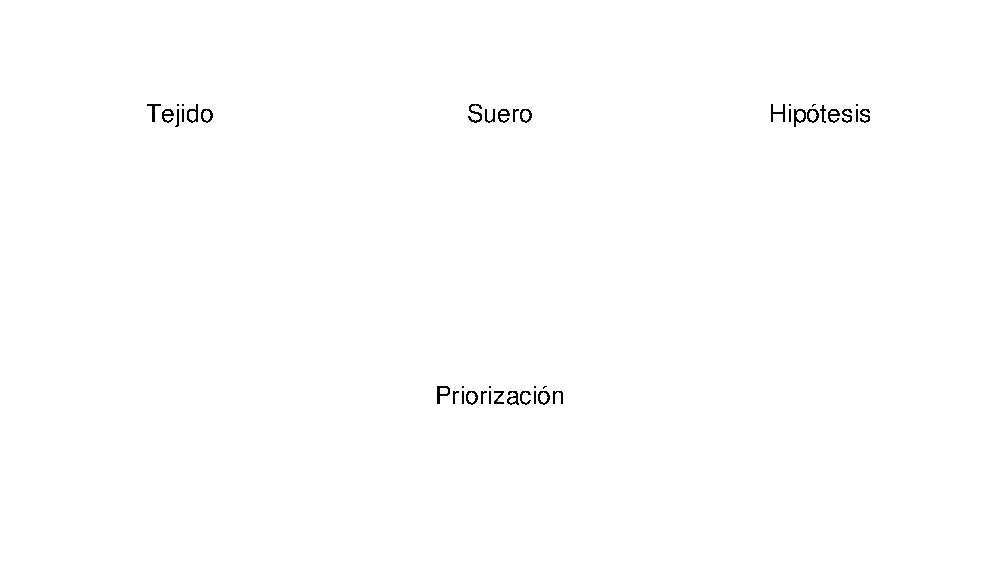
\includegraphics[width=0.92\textwidth]{figures/f01.pdf}
\caption{Cuatro bloques de la corrida: tejido, suero, hipótesis y priorización. El trazo une el orden de lectura. No representa una proteína que pasa del tumor a la sangre.}
\label{fig:mapa}
\end{figure}
\fuente{\texttt{scripts/v3/exportar\_sitio\_v3\_7.py}, figura \texttt{f01}, a partir de \texttt{results/v3\_7/}.}
\todojd{escribe tu interpretación de la figura \ref{fig:mapa}.}

\section{Tejido}
\begin{itemize}
\item Signo del tumor primario, Tanaka frente a CPTAC: \TejidoNum\ de \TejidoDen.
\item Metástasis hepática frente a mucosa: \TejidoMetaNum\ de \TejidoMetaDen.
\item Cobertura: \CoberturaNum\ de \CoberturaDen. Veredicto de H1: \HunoVeredicto.
\item Concordancia de NES: \GoConNum\ de \GoConDen.
\end{itemize}
\begin{figure}[ht]
\centering

\includegraphics[width=0.84\textwidth]{figures/f05.pdf}
\caption{Cada punto es un gen de la tabla de H7 medido también en Tanaka. El eje horizontal es el \(\log_2\)FC de CPTAC y el vertical, el de Tanaka.}
\label{fig:tejido}
\end{figure}
\fuente{\texttt{results/v3\_7/}, figura \texttt{f05}.}
\todojd{escribe tu interpretación de la figura \ref{fig:tejido}. No afirmes que el signo compartido localiza una muestra.}

\begin{figure}[ht]
\centering

\includegraphics[width=0.84\textwidth]{figures/f07.pdf}
\caption{Cada punto es un término con FDR de CPTAC dentro del umbral y con NES en Tanaka.}
\label{fig:go}
\end{figure}
\fuente{\texttt{results/v3\_7/go\_tejido.json}, figura \texttt{f07}.}
\todojd{escribe tu interpretación de la figura \ref{fig:go}. Un ORA de cero términos en Tanaka no es ausencia de biología: Tanaka tiene \GoTanakaSuben\ términos ORA que suben y \GoTanakaBajan\ que bajan, y \GoTanakaGsea\ con GSEA.}

\section{Suero}
\begin{table}[ht]
\caption{Celda preregistrada del suero, CP frente a CN}
\label{tab:celda}
\begin{tabular}{lr}
\toprule
Clase & Proteínas \\
\midrule
Diferentes & \SueroDif \\
Equivalentes & \SueroEq \\
Indeterminadas & \SueroInd \\
Total & \SueroN \\
\bottomrule
\end{tabular}
\end{table}
\fuente{\texttt{results/v3\_7/suero\_embudo.json}, campo \texttt{celda\_preregistrada}.}
\todojd{El cero no lleva un segmento inventado. No escribas que la equivalencia estadística es identidad biológica.}

\begin{figure}[ht]
\centering
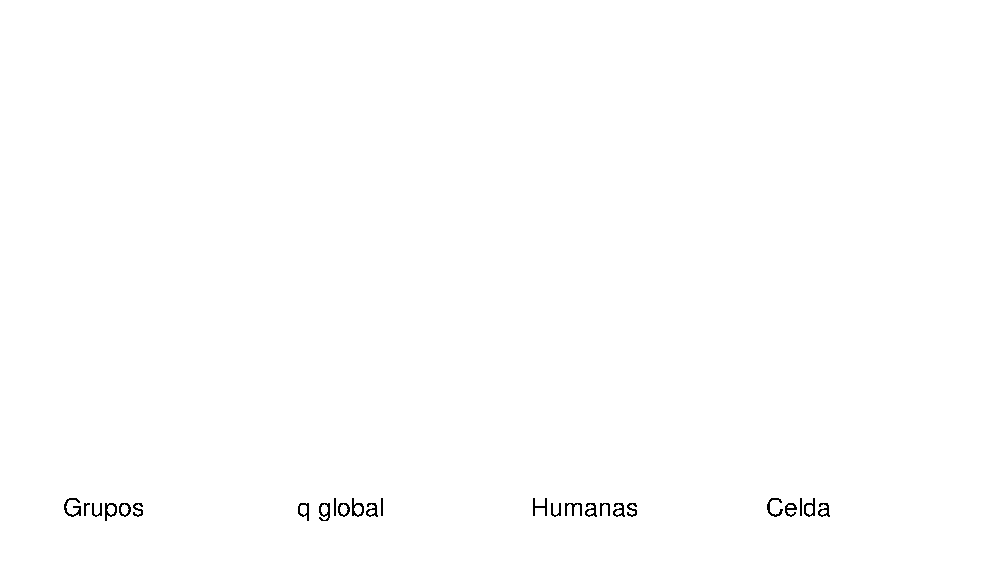
\includegraphics[width=0.92\textwidth]{figures/f02.pdf}
\caption{Embudo del suero. Alturas: \EmbudoGrupos\ grupos, \EmbudoQ\ con el filtro global, \EmbudoHumanos\ humanas y la celda de \SueroN.}
\label{fig:embudo}
\end{figure}
\fuente{\texttt{results/v3\_7/suero\_embudo.json}, figura \texttt{f02}.}
\todojd{escribe tu interpretación de la figura \ref{fig:embudo}.}

\begin{figure}[ht]
\centering
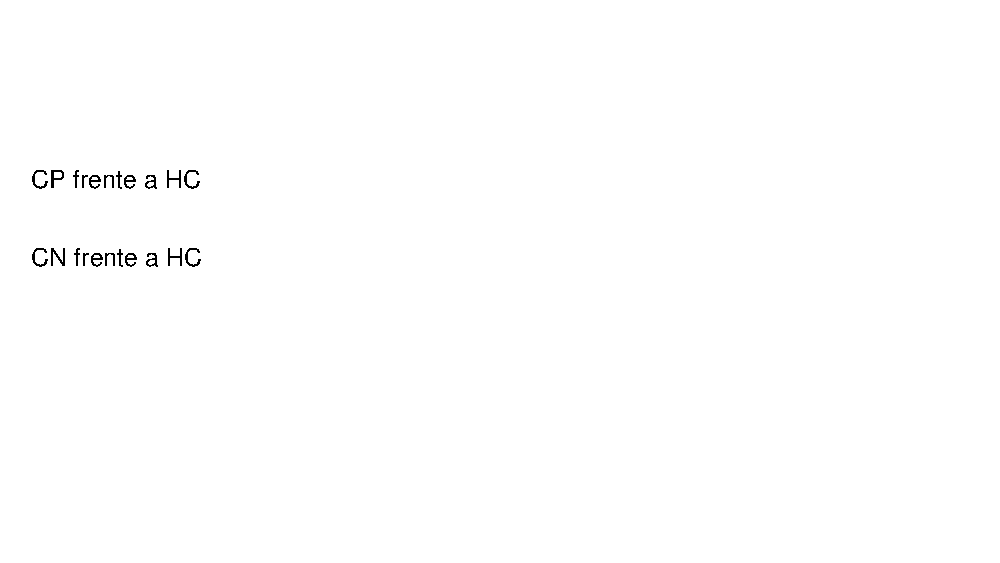
\includegraphics[width=0.84\textwidth]{figures/f03.pdf}
\caption{La barra superior es CP frente a CN. Las de abajo son los contrastes con HC, medido aparte: \HcCpDif\ diferentes en CP y \HcCnDif\ en CN. HC no decide la pregunta.}
\label{fig:hc}
\end{figure}
\fuente{\texttt{suero\_k4\_crc\_sanos.tsv} y \texttt{suero\_k4\_cn\_sanos.tsv}, figura \texttt{f03}.}
\todojd{escribe tu interpretación de la figura \ref{fig:hc}. No llames sanos a CN.}

\section{Calidad, orden y modelos}
\begin{itemize}
\item Preanalítica: estado \PreEstado. Crudos válidos: \PreCrudos. Con fecha: \PreFecha. AUC del orden: \PreAuc. p exacta de Mann-Whitney: \(1{,}5\times 10^{-11}\). Es el valor de \texttt{cifras.tex} (\texttt{\textbackslash PreP}); va en fórmula porque la fuente no tiene el signo de exponente.
\item M2, todas las proteínas: AUC \MlTodas. M3, solo calidad: \MlCalidad. M5, sin la calidad: \MlSinCalidad, p \MlSinCalidadP.
\item M1: \MlHumana. M4, coagulación: \MlCoagulacion. M6: \MlPca.
\end{itemize}
\begin{figure}[ht]
\centering
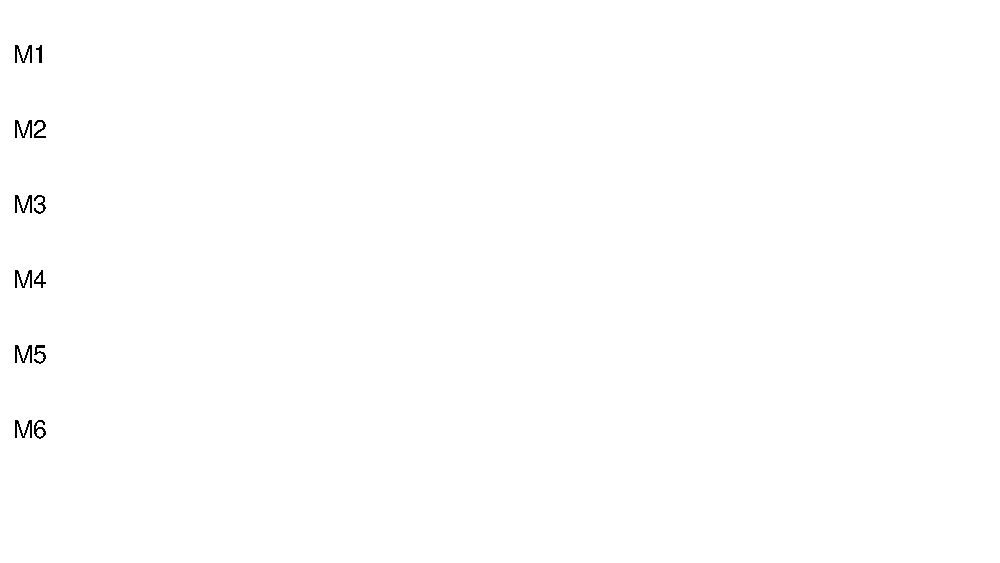
\includegraphics[width=0.84\textwidth]{figures/f08.pdf}
\caption{AUC fuera de pliegue de M1 a M6. La línea discontinua es el percentil 95 del nulo de K5.}
\label{fig:auc}
\end{figure}
\fuente{\texttt{results/v3\_7/ml\_suero\_permutacion.json}, figura \texttt{f08}.}
\todojd{escribe tu interpretación de la figura \ref{fig:auc}. No presentes el AUC como sensibilidad ni como especificidad de un examen.}

\begin{figure}[ht]
\centering
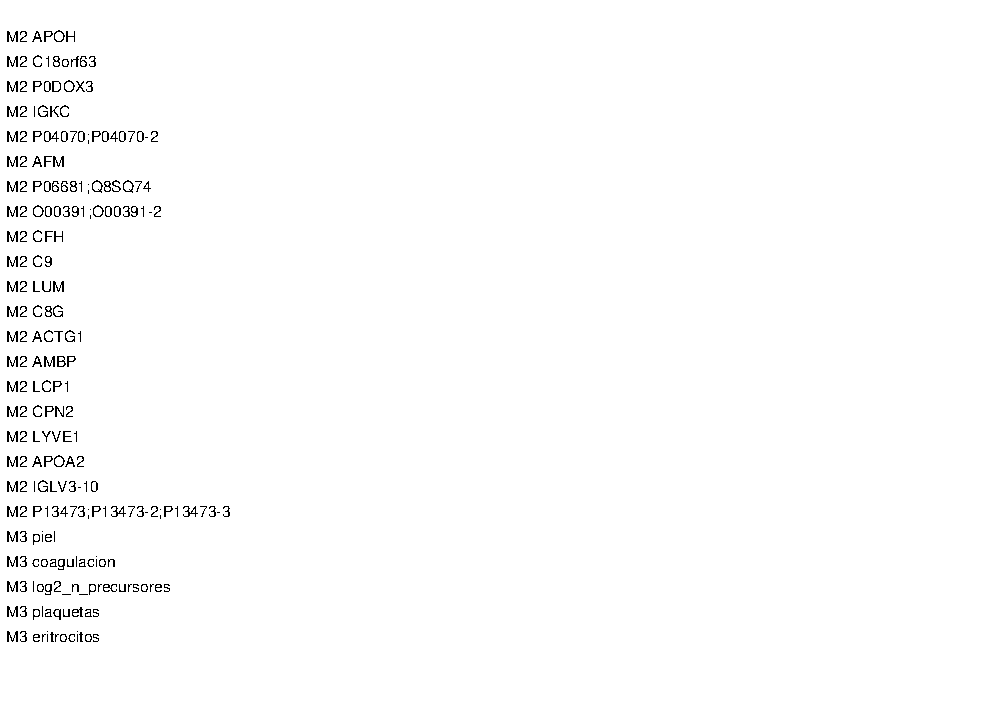
\includegraphics[width=0.78\textwidth]{figures/f09.pdf}
\caption{Media del valor absoluto de SHAP en M2 y en M3. M3 usa las variables de calidad que trae el fichero.}
\label{fig:shap}
\end{figure}
\fuente{Figura \texttt{f09}.}
\todojd{escribe tu interpretación de la figura \ref{fig:shap}.}

\section{Hipótesis y priorización}
\begin{table}[ht]
\caption{Estado de las hipótesis en la corrida firmada}
\label{tab:hipotesis}
\begin{tabular}{llp{7.2cm}}
\toprule
Hipótesis & Estado & Cifra que sí está \\
\midrule
H5 & \HcincoEstado & \HcincoUniverso\ genes en el universo principal. Fracción pan-carcinoma 0,119. Clasifica 624 proteínas. \\
H6 & \HseisEstado & No informa a favor ni en contra. \\
H7 & \HsieteEstado & Álvez 2023: AUC \HsieteAlvez. HPA: AUC \HsieteHpa. Secundario: \HsieteSec, con vector en \HsieteNEsm\ y \HsieteOmitidas\ omitidas. \\
H8 & \HochoEstado & \HochoTumorales\ tumorales epiteliales en \HochoUniverso. \\
H9 & \HnueveEstado & No decide la tesis. \\
H10 & \HdiezEstado & \HdiezN\ proteínas. \\
\bottomrule
\end{tabular}
\end{table}
\fuente{JSON \texttt{h5} a \texttt{h10} de \texttt{results/v3\_7/}.}
\todojd{El intervalo de Álvez es 0,381 a 0,584 (53 y 73) y el del HPA es 0,353 a 0,573 (53 y 63). Papier 2024 queda no evaluable: 1 y 125. Escribe eso solo si usas H7.}

\begin{itemize}
\item Pasos de priorización: \PrioriPasoUno, \PrioriPasoDos, \PrioriPasoTres, \PrioriPasoCuatro, \PrioriPasoCinco, \PrioriPasoSeis\ y \PrioriPasoSiete.
\item Del paso 5, \PrioriBajan\ bajan en CPTAC y \PrioriSuben\ suben.
\item Multiverso: \MultiSuero\ celdas de suero, \MultiMl\ de aprendizaje, \MultiDif\ con alguna proteína diferente.
\end{itemize}
\begin{figure}[ht]
\centering

\includegraphics[width=0.84\textwidth]{figures/f04.pdf}
\caption{Rejilla de \MultiSuero\ celdas. El trazo discontinuo marca las que tienen alguna proteína diferente. No es una cohorte nueva.}
\label{fig:multi}
\end{figure}
\fuente{\texttt{results/v3\_7/multiverso\_resumen.json}, figura \texttt{f04}.}
\todojd{escribe tu interpretación de la figura \ref{fig:multi}.}

\begin{figure}[ht]
\centering
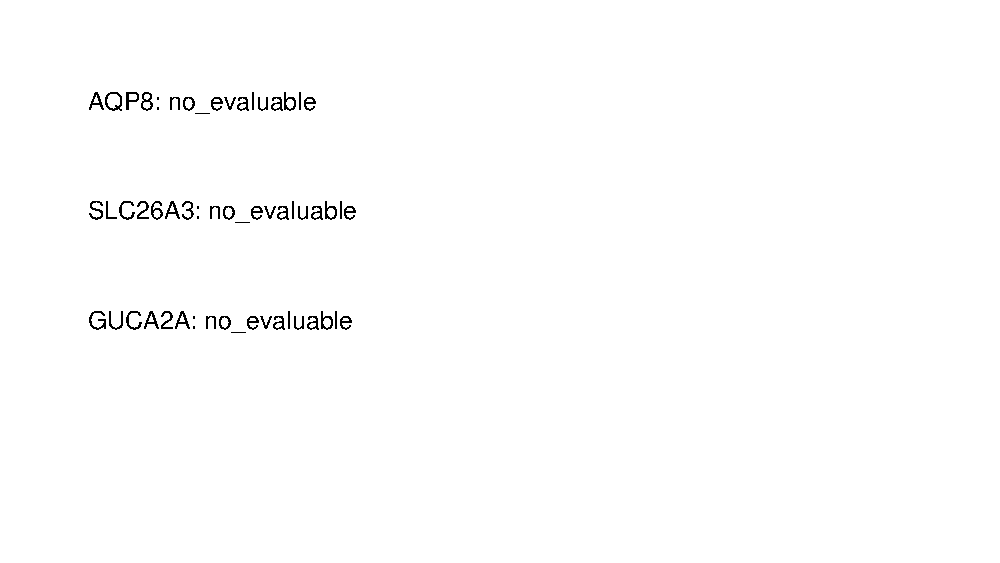
\includegraphics[width=0.7\textwidth]{figures/f06.pdf}
\caption{Controles de tejido no medibles. AQP8, GUCA2A y SLC26A3 quedan con trazo discontinuo porque el fichero no los da para la prueba.}
\label{fig:controles}
\end{figure}
\fuente{Figura \texttt{f06}. [PENDIENTE: verificar en \texttt{results/v3\_7/} el veredicto de CA1 antes de escribirlo en la prosa. El anexo viejo decía «CA1 pasa» y no se copió aquí.]}
\todojd{escribe tu interpretación de la figura \ref{fig:controles} solo con el fichero que abras.}

\chapter{Discusión}
% fuente: results/v3_5/ml_celda_preregistrada.json
% fuente: results/v3_3/ml_suero_modelos.tsv
% fuente: results/v3_5/preanalitica_v3_5.json
% fuente: results/v3_5/h8_carga_tumoral.json
% fuente: results/v3_5/h6_origen_celular.json
% fuente: results/v3_5/h7_visibilidad_en_sangre.json

\section{La preanalítica}
La lección central está en la calidad de la muestra. La piel, la coagulación, los eritrocitos y las plaquetas separan grupos que el contraste de proteínas no separa \cite{geyer2019}. Un lote de adquisición puede producir la misma apariencia de biología \cite{leek2010}. En \texttt{preanalitica\_v3\_5.json} hay fecha para \VcincoPreFecha\ de \VcincoPreCrudos\ crudos. El estado es \VcincoPreEstado. Las corridas legibles van por bloques. Eso no demuestra que el titular del suero sea un efecto de lote, y tampoco lo descarta para los crudos sin fecha.

La coagulación puede ser del tubo y del tiempo hasta centrifugar. También puede ser del cáncer, porque el tumor activa la coagulación. La piel es de manipulación. Esas dos lecturas no se pueden separar con estos ficheros.

\section{El resultado negativo}
\VcincoSueroDif\ de \VcincoSueroN\ proteínas separan el cáncer de la colonoscopia negativa. \VcincoSueroInd\ quedan indeterminadas. Con el tamaño de esta cohorte, no detectar una diferencia no equivale a demostrar que la diferencia no existe. Las \VcincoSueroEq\ equivalentes sí descartan el cambio que la regla fija. Esa distinción es la contribución del contraste.

\section{Coherencia biológica}
SAA1, LBP y LRG1 suben frente a personas sanas y no frente a la colonoscopia negativa. Son proteínas de fase aguda: señal de inflamación del huésped, no específica del tumor \cite{gabay1999}. CEACAM5 sube en el tejido y no aparece como diferencia en este suero. Su uso clínico es el seguimiento, no el cribado \cite{locker2006}. H8 queda en \VcincoHocho. Muchos casos de esa cohorte son estadio IV y las proteínas hepáticas salen por la lista de ruido. Un DIA sin depleción no alcanza la profundidad que la regla pide \cite{hermoso2026}.

\section{Otros estudios}
Álvez, Papier, Wannberg y Hermoso-Durán preguntan cosas distintas. Unos miden sangre de personas sanas o de riesgo prospectivo. Otro mide estadio en suero. No se comparan áreas bajo la curva entre diseños distintos. H7 queda en \VcincoHsiete\ dentro de sus propias reglas. El acuerdo entre recursos es bajo. Los recursos no miden lo mismo.

\section{Limitaciones}
El suero tiene un grupo pequeño y un solo centro. Las cohortes públicas no traen tejido y sangre de la misma persona. Parte de los controles del tejido no se detecta. La preanalítica tiene \VcincoPreFecha\ de \VcincoPreCrudos\ crudos. H6 tiene la tabla degenerada. La independencia de los recursos de H7 no está comprobada. H9 usa un instrumento por proteína. Ninguna de esas frases propone un examen.

\section{Qué diseño lo evitaría}
Un orden de adquisición aleatorizado, paneles de calidad escritos de antemano y una cohorte externa de personas con síntomas, con tejido y sangre de la misma persona. Eso sigue siendo fase 1 de Pepe hasta que una cohorte nueva, fijada de antemano, repita el resultado \cite{pepe2001}.

\chapter{Conclusiones y recomendaciones}

\section{Conclusiones}
Las conclusiones responden a los objetivos.

\begin{itemize}
% fuente: results/v3/k1_etiquetas.json
\item Entre las 688 proteínas certificadas, el primario de Tanaka coincide en signo con CPTAC en 116 de 118. El intervalo va de 0,940 a 0,998. La metástasis hepática frente a la mucosa coincide en 93 de 106. La lectura anterior, con la metástasis leída como tumor, era 104 de 119 y se conserva con ese nombre. En el universo más amplio del 31 de octubre, 687 de 874 genes coinciden en signo y la correlación de Pearson es 0,83. Son dos cuentas distintas.
% fuente: results/v3/k4_potencia.json
% fuente: results/v3/k6_presencia.tsv
\item En el suero, ninguna de las 876 proteínas separa el cáncer de la colonoscopia negativa con el corte de 1,5 veces. De ellas, 145 tienen ese cambio descartado y 731 quedan indeterminadas. SAA1, LBP y CHMP4A separan el cáncer de las personas sanas. Las dos primeras se leen como respuesta del huésped. CHMP4A tiene 13, 4 y 3 presencias en los tres grupos de 20, y no se imputa. La fracción de albúmina y la coagulación difieren entre grupos.
% fuente: results/v3/k5_auc.json
\item El máximo del área bajo la curva del catálogo, 0,9375, tiene p = 0,0245 frente a 10\,000 permutaciones. La media de ese nulo es 0,843. No es una prueba diagnóstica.
\item Los procesos GO del tejido casi no están medidos en este suero. Los doce a trece términos del cierre del 31 de octubre no se han vuelto a evaluar con 10\,000 permutaciones. Esa cláusula queda en curso.
\item Los péptidos mutados descritos por Rai, Xiang y Hembrough no se confirman ni se rechazan con esta matriz. El resultado de ese objetivo es el límite del método.
\item La especificidad de órgano, el origen celular, la visibilidad en sangre, la carga tumoral, la dirección causal y la especificidad frente a otras enfermedades están preregistradas. Esta versión no les asigna un número.
\end{itemize}

En conjunto, el cambio de proteínas del tumor se repite entre tejidos y en este suero no aparece como una señal propia del cáncer. El trabajo sirve para responder esa pregunta. No sirve para proponer un examen de sangre.

\section{Recomendaciones}
Se recomienda repetir BAIAP3 en otra cohorte con colonoscopia negativa, con más de veinte personas por grupo y con el antígeno carcinoembrionario de la misma persona.

Se recomienda copiar, del suplemento de Rai y colaboradores, las secuencias de los 19 péptidos y rebuscarlas en crudos independientes, con control de falsos por clase de péptido. Ese resultado no se anticipa con un número.

Se recomienda medir CEACAM5 de forma dirigida en suero, que es la escala del panel de Ögren y colaboradores, no la de esta matriz DIA.

Se recomienda emparejar la tabla de muestras de Lesur y colaboradores con las columnas de PXD036594 antes de usar ese plasma.

Se recomienda aplicar el suplemento de origen tisular de Malmström y colaboradores cuando esté disponible como tabla. Hoy la ficha usa secreción y Gene Ontology.

Se recomienda incorporar, cuando exista, tejido y sangre de la misma persona. Estas matrices no los traen juntos.

\chapter{Anexos}

\section{Fuentes confirmadas}
La tabla~\ref{tab:fuentes} lista las fuentes cuyo DOI se confirmó en Crossref el 31 de octubre de 2026. El título del registro coincide con la cita. La referencia completa, en APA 7, está al final del documento. Si la tabla pasa de página, se repite el encabezado y la leyenda de continuación.

\begin{longtable}{@{}p{6.2cm}p{1.6cm}p{6.4cm}@{}}
\caption{Fuentes confirmadas en Crossref el 31 de octubre de 2026}
\label{tab:fuentes}\\
\toprule
Fuente & Año & DOI \\
\midrule
\endfirsthead
\caption*{Tabla \thetable: (Continuación)}\\
\toprule
Fuente & Año & DOI \\
\midrule
\endhead
\bottomrule
\endfoot
Ashburner et al. & 2000 & 10.1038/75556 \\
Benjamini y Hochberg & 1995 & 10.1111/j.2517-6161.1995.tb02031.x \\
Congreso de la República de Colombia & 2010 & Ley 1384 de 2010 \\
Cox y Mann & 2008 & 10.1038/nbt.1511 \\
Dhami et al. & 2026 & 10.1002/prca.70041 \\
García-Foncillas et al. & 2026 & 10.51643/22562915.853 \\
Hembrough et al. & 2026 & 10.1158/1538-7445.am2026-7710 \\
Jumper et al. & 2021 & 10.1038/s41586-021-03819-2 \\
Lesur et al. & 2023 & 10.1021/acs.jproteome.2c00575 \\
Li et al. & 2024 & 10.1038/s41467-024-44911-1 \\
Malmström et al. & 2025 & 10.1016/j.cell.2025.03.013 \\
McCarthy y Smyth & 2009 & 10.1093/bioinformatics/btp053 \\
Ögren et al. & 2026 & 10.1186/s12943-026-02654-1 \\
Rai et al. & 2025 & 10.1021/acs.jproteome.5c00285 \\
Robles et al. & 2024 & 10.1371/journal.pcbi.1011828 \\
Seo et al. & 2026 & 10.1002/jev2.70278 \\
Smyth & 2004 & 10.2202/1544-6115.1027 \\
Subramanian et al. & 2005 & 10.1073/pnas.0506580102 \\
Tanaka et al. & 2024 & 10.1016/j.celrep.2024.113810 \\
Uhlén et al. & 2015 & 10.1126/science.1260419 \\
Vasaikar et al. & 2019 & 10.1016/j.cell.2019.03.030 \\
Verathamjamras et al. & 2023 & 10.1186/s12014-023-09407-y \\
Xiang et al. & 2026 & 10.1016/j.xgen.2025.101062 \\
Yu et al. & 2026 & 10.1186/s12885-026-15547-9 \\
Zhang et al. & 2014 & 10.1038/nature13438 \\
\end{longtable}
\fuente{Crossref, consulta del 31 de octubre de 2026. La Ley 1384 de 2010 no tiene DOI.}

\section{Identificadores que no entran}
No entran en las referencias, porque el 31 de octubre de 2026 el identificador no abrió un artículo: 10.1016/j.xcrm.2025.101689, la cita mal formada de ENCODE y el identificador 10.64898/2026.08.30.26361622. Los preprints de Lee, Tan y Ramsbottom pueden ir a un anexo futuro, marcados como no revisados por pares. No se usan como evidencia de un resultado.

\section{Tablas de la corrida del 6 de noviembre}
Los números nuevos de esta versión salen de \texttt{results/v3/}. El contraste de tejido está en \texttt{k1\_etiquetas.json} y en \texttt{k1\_comparacion\_contrastes.tsv}. Las clases del suero están en \texttt{k4\_potencia.json}. El nulo del área bajo la curva está en \texttt{k5\_auc.json}. La presencia de CHMP4A está en \texttt{k6\_presencia.tsv}. El control técnico está en \texttt{k7\_control\_tecnico.json}. El cambio respecto de la versión anterior está en \texttt{changelog\_numeros.tsv}. El preregistro es \texttt{config/preregistro\_v3.yaml}. La auditoría y las enmiendas están en \texttt{docs/auditoria\_v3.md} y \texttt{docs/enmiendas\_v3.md}.

\section{Nota sobre la correlación 0,104}
La correlación 0,104, con 56\,\% de igual signo y 1\,993 proteínas, es una estadística anterior. Usó otra lectura de las columnas de PXD034575. La correlación 0,83 es la del primario, ya en log2, contra CPTAC, con 874 genes. Se citan juntas, cada una con su $n$. No se presenta 0,83 como la corrección de 0,104. Ninguna de las dos es tejido contra sangre. La concordancia de tejido hacia plasma de la versión certificada sigue siendo 0,488 (42 de 86).


\cleardoublepage
\nocite{*}
\printbibliography[heading=bibintoc,title={Referencias bibliográficas}]

\end{document}
